% !TEX encoding = MacOSRoman
\chapter{System Design}
\label{systemschapter}

This chapter presents the design and architecture of \nplh, an online application that serves as a platform for facilitating pet-to-family reunification through the activities of digital volunteers.  The beginning of this chapter discusses the various interaction design requirements we\footnote{I use the pronouns ``we'' or ``us'' deliberately in this chapter to refer to work done in collaboration with Mario Barrenechea and Joanne White \cite{sdc}.}generated during prototyping this system and their relationship to other system components.  The following sections are focused on detailing the software architecture of the system.

\section {Application Features and Interface Design}

\nplh{} is a system for use by digital volunteers.  Examining the activities of digital volunteers through the lens of the Data Scouts framework allows us to elicit system requirements.  Table~\ref{table:dsreqs} lists the primary tasks we envisioned being facilitated by the system.

\begin{table}[htb] 
    \caption[Tasks facilitated by the system]{
	This table shows the most prominent tasks facilitated by the system, divided by the role of the user performing them.
	}
    \begin{center}
    \begin{tabular}{||c|l||} \hline
	{\em Data Scouts Role} & Tasks \\  \hline \hline
	Data Scout  & Reporting lost or found pets. \\ \hline
	Consolidator & Matching lost pet reports with found pet reports. \\ \hline
	Checker & Verifying matches proposed by consolidators, editing pet reports. \\ \hline
	\end{tabular}
   \\ \rule{0mm}{5mm}
	\end{center}
	\label{table:dsreqs}
\end{table}

Of these tasks, the matching task facing the consolidators who use the system is the most complex to design for, and it is where we focused most of our efforts.  The matching task is difficult for a variety of reasons.  There are technical challenges to overcome, the most difficult of which is that the size of the search space for possible matches is very large; this is the motivating factor behind the inclusion of machine learning components in the system.  Even with assistance from these components, users of the system will still need to sift through several candidates before completing the matching task.  Finally, because the machine learning components act in collaboration with users (and because we cannot expect them to be perfectly accurate in completing their tasks), we must provide tools for users to manually complete the matching task. 

There are also several social challenges that have been addressed during the design of this system.  Many of these problems are related to user demographics; although consolidators all engage in the same task, they are likely to be a highly diverse group in terms of age, background, enthusiasm, and technical experience.  In addition, because collaboration between volunteers is a key component to the completion of virtually all the tasks facilitated by the system, the system must provide a collaboration mechanism and a social networking system.  

The solutions chosen to address these challenges motivate the key features of \nplh, each of which are discussed individually in the following sections.

\subsection {Accessible User Interface}

Because of the diversity of the projected users for \nplh, our design solution must be accessible to users in a variety of ways.  Part of our initial design work was in generating personas to model the users of the system: these personas included a wide range of profiles, ranging from elementary students to young adults to senior citizens\cite{sdc}.  As such, the design of our user interfaces is motivated by these goals:

\begin{itemize}
  \item{} The default work flow to complete tasks, especially the matching task, must be intuitive and simple to complete.
  \item{} The tool must provide alternate work flows to accommodate the different levels technical expertise and motivation that users may possess; this is to say that the depth and complexity of the interaction available to users must vary based on these factors.
\end{itemize}

In pursuing these design goals we have created several interfaces in an iterative manner.  Our prototype interfaces have all been focused on the work flow for the matching task.  The design changes made from iteration to iteration have been informed by user centered design techniques (generally cognitive walkthroughs and ``thinking aloud'' exercises with users).  Figures~\ref{fig:design1} and~\ref{fig:design2} show the evolution of the interface design from low to higher fidelity prototypes.

\begin{figure}[htbp]
    \begin{center}
	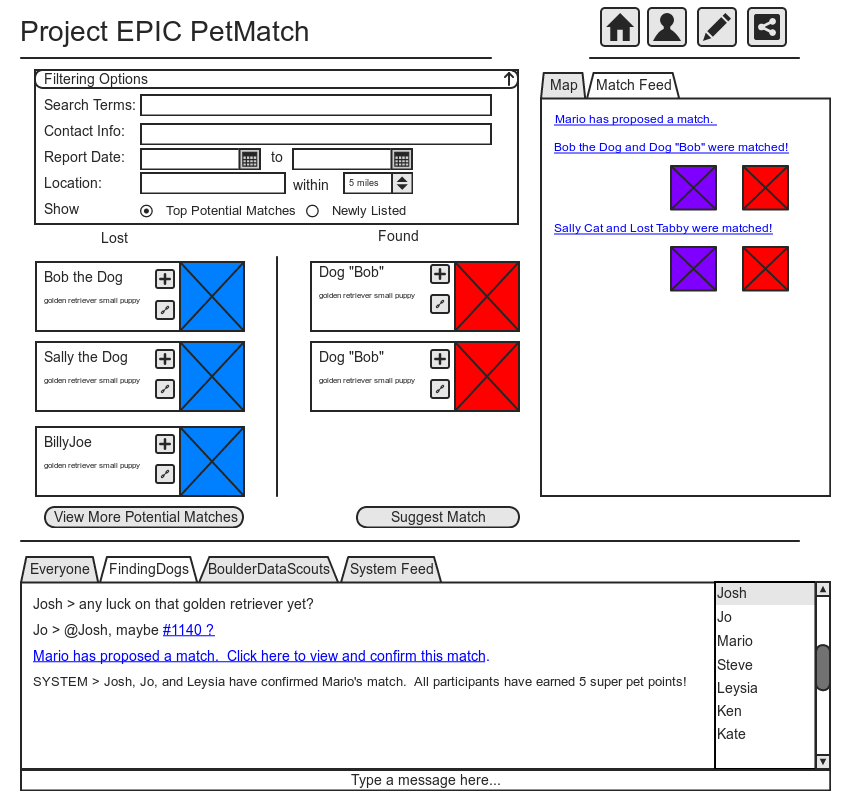
\includegraphics[width=150mm]{figs/design1.png}
    \end{center}
        \caption[First Interface Prototype]{
        Low-fidelity mockup of an interface to complete the matching task.
	}
	 \label{fig:design1}
\end{figure}

\begin{figure}[htbp]
    \begin{center}
	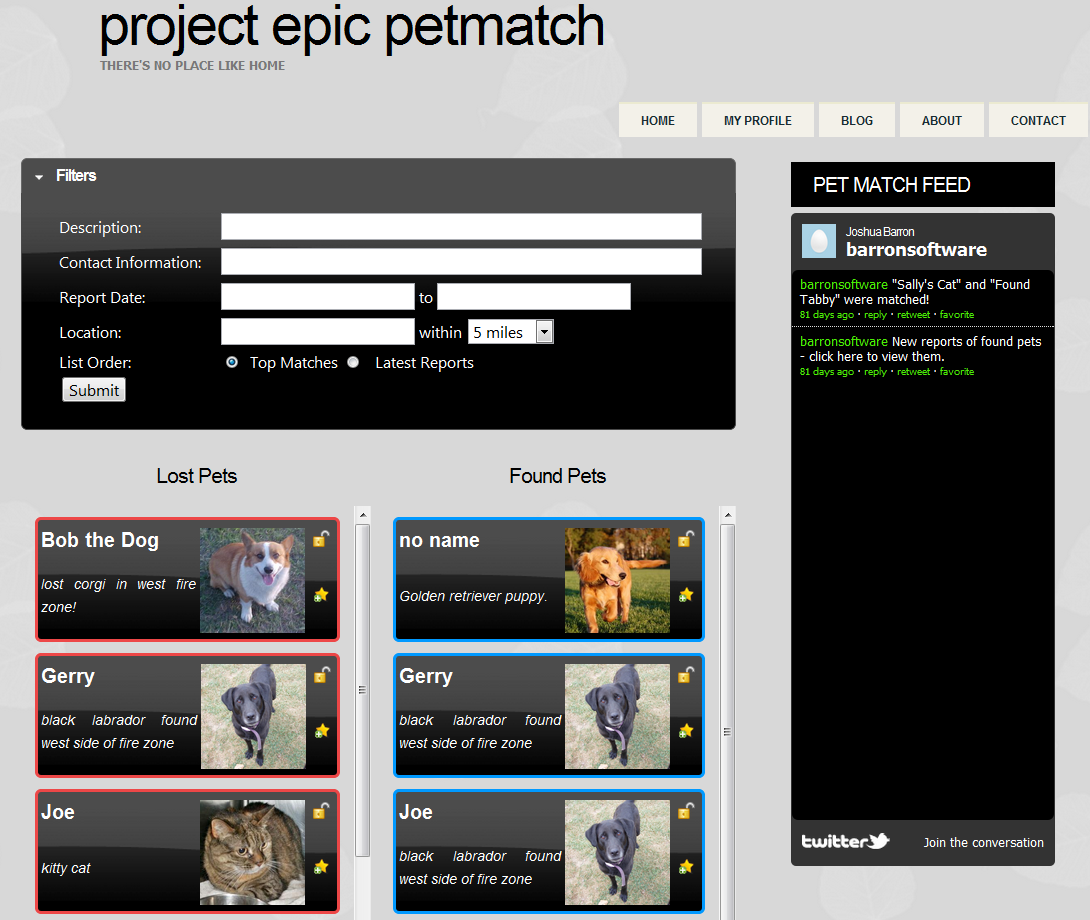
\includegraphics[width=150mm]{figs/design2.png}
    \end{center}
        \caption[Second Interface Prototype]{
        Medium-fidelity mockup of an interface to complete the matching task.
	}
	 \label{fig:design2}
\end{figure}

The design of the user interfaces for \nplh{} is an ongoing process.  After completing our initial prototyping \cite{sdc} and user testing, we discovered problems with the initial design of the matching interface:

\begin{itemize}
  \item{} Virtually all participants ignored the advanced search capabilities, instead favoring visually browsing pet reports.
  \item{} Many participants needed to temporarily store pet reports (that they considered match candidates) while considering other pet reports for a match.
  \item{} The two-column design (see Figure~\ref{fig:design2} was not optimal for the matching task, as participants often just picked a pet report from one side (indeed, our testing scenarios were even set up this way) and then, of course, completely ignored that column for the duration of the task.  This meant that valuable screen real estate was going to waste in addition to being a source of confusion for users.
\end{itemize}

Solving these problems is the subject of our ongoing design work.  We have labored to separate the interfaces for the matching task so that they more closely match the observed work flow of testing participants; we now have a separate interface for selecting a pet to ``work'' on and another interface for finding a match for that pet.  The new matching interface is much more visually oriented, drawing design inspiration from sites such as Pinterest, and incorporates new functionality to allow users to preserve their work in the form of a temporary workspace which holds candidates that the user has selected.  Figures~\ref{fig:design3} and~\ref{fig:design4} display early prototypes of these new interfaces.

\begin{figure}[htbp]
    \begin{center}
	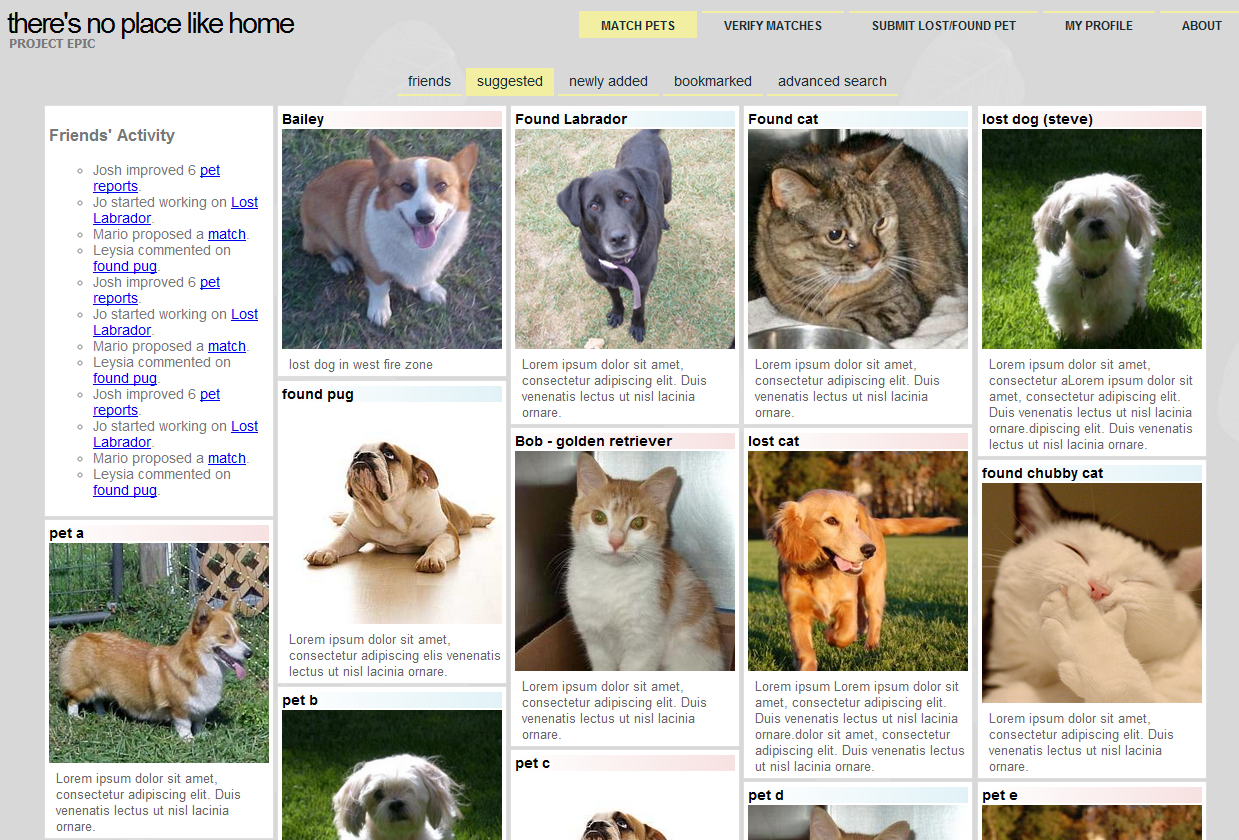
\includegraphics[width=150mm]{figs/design3.png}
    \end{center}
        \caption[Third Interface Prototype: selecting a pet to work on]{
        Medium-fidelity mockup of the pet selection interface; a user selects a pet to work on the matching activity via this interface.
	}
	 \label{fig:design3}
\end{figure}

\begin{figure}[htbp]
    \begin{center}
	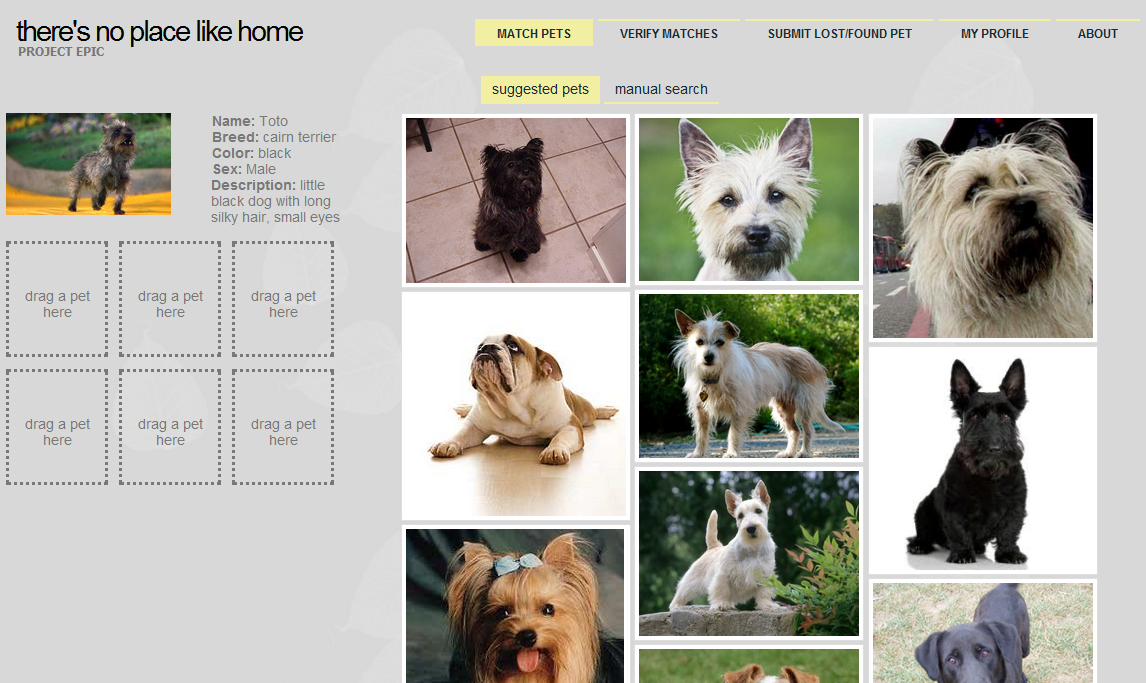
\includegraphics[width=150mm]{figs/design4.png}
    \end{center}
        \caption[Fourth Interface Prototype: finding a match for a pet]{
        Medium-fidelity mockup of an interface to complete the matching task, utilizing a new workspace area (for drag-and-drop actions) and increased screen real estate.
	}
	 \label{fig:design4}
\end{figure}

\subsection {Collaboration and Social Capital}

Collaboration and networking are key to facilitating the crowd work performed by digital volunteers.  Because digital volunteers have been shown to connect to each other both via pre-existing connections as well as connections which emerge around the completion of a task \cite{starbird:voluntweeters}, this social networking mechanism should honor existing social connections as well as those that are forged during an event. \nplh{} does this by allowing users to access the system via their Facebook or Twitter account; alternatively, the user can also rapidly create a site-specific account.  In addition to providing a quick authentication mechanism, the system can also use this information to import the user's existing social connections.

Supporting social networks provides a backbone to the social features of the system, but an active mechanism to support collaboration is still needed.  \nplh{} therefore implements a chat room functionality that lives at the bottom of every interface in the application.  Chat rooms allow users to connect with their social network and coordinate as they complete tasks within the system.  Chat rooms are automatically created for groups of people working on specific pet reports, and the chat interface is present at the bottom of every user interface in the system.  Logs of chat activity for these rooms are attached to the corresponding pet report and saved as they represent valuable contextual information for future work with that pet.

Chat rooms are also designed to support contextual links (i.e., a user can easily insert a link to an artifact, such as a pet report, into a chat message) to facilitate quicker collaboration.  In addition, automated messages are sent to relevant users when certain artifacts are created within the system - for example, a user might be prompted to vote on a match proposed by one of his or her friends.  This is another key feature of the system which facilitates rapid verification of pet matches by on-task populations of users.

In order to provide some regulation to the community activity which takes place during an event via the system, as well as to provide an incentive mechanism and a potentially interesting feature for the machine learning components of the system, a social capital mechanism is also present within the system.  Users earn social capital (represented as a numerical value) for completing various actions within the system, such as submitting a pet report, editing a pet report, proposing a match for a pet report, or voting on a proposed match for a pet report.  Furthermore, if a user is the creator of an artifact within the system (such as a pet report or a proposed match), the social capital of that user can be affected when other users take actions on that artifact (i.e., voting on on a proposed match).  Social capital is a public indicator of the status of an individual within the community, and in addition, the system makes use of it to automatically grant administrative capabilities to the highest rated users.

\section {Software Architecture}

I have discussed the system design and key features of \nplh{} in the previous sections of this chapter.  
This portion of the chapter discusses the architectural design and implementation of the software which makes up \nplh.  The system is implemented primarily as a web application under the {\em Django} framework.  Data is managed via document collections in a {\em MongoDB} store.

The following sections discuss the various data artifacts managed by the system, the deployment of the system, and the implementation of the Django applications and other Python components which make up the system.

\subsection {Artifacts and Data Management}

Although the interactions facilitated by the system are rich and complex, the data artifacts generated by users and managed by the system are relatively simple.  Artifacts are generally related to either users and user activity or pet reports.  Table~\ref{table:artifacts} describes the various artifacts managed by the system.

\begin{table}[htb]
    \caption[Artifacts]{
	This table details the artifacts tracked by the system.
	}
    \begin{center}
    \begin{tabular}{|| c | l | p{7cm} ||} \hline
	{\em Artifact} & \em Generator & Description \\  \hline \hline
	{\tt Pet} & Data Scout & Represents a lost or found pet reported to the system. \\ \hline
	{\tt Match} & Consolidator & Describes a proposed match between one lost pet and one found pet. \\ \hline
	{\tt User} & Any & Represents a user of the system and tracks work items in addition to authentication information.  \\ \hline
	{\tt Chat} & Any & Represents a chat room in the system - can be linked to a specific {\tt Pet}. \\ \hline
	\end{tabular}
   \\ \rule{0mm}{5mm}
	\end{center}
	 \label{table:artifacts}
\end{table}

Instead of storing data in a relational database, which is the typical design choice in client-server applications, \nplh{} makes use of MongoDB\footnote{http://www.mongodb.org/}, a document-oriented data store.  The reasons for this design decision are detailed in the following section.

Utilizing a document-oriented data store allows the artifacts tracked by the system to be stored in a format which is very similar to their conceptual structure.  Documents can aggregate complex data structures without resorting to linking, which leads to a design that is fairly concise.  The decision to make an artifact or its properties a top-level document in the collection usually comes down to whether or not doing so would prevent data replication rather than concerns about normalization and performance that are common in relational designs.  The design of a document as an artifact's representation is akin to doing object-oriented design; so much, in fact, that I choose to detail the implementation of the system's database as a class diagram in Figure~\ref{fig:db}.

\begin{figure}[htbp]
    \begin{center}
	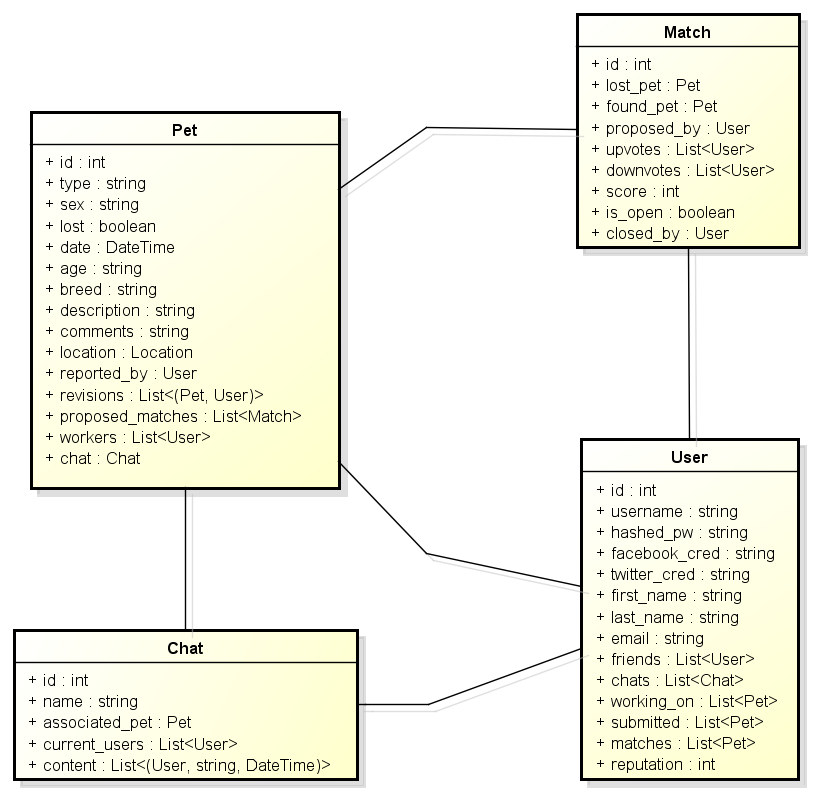
\includegraphics[width=150mm]{figs/artifacts.png}
    \end{center}
        \caption[Database Design]{
        Object-oriented database design for \nplh{}.  Note that there are several associations between several of the artifacts, and that this diagram does not detail each association; refer to the contents of each artifact for more detail.
	}
	 \label{fig:db}
\end{figure}

\subsubsection {Data Management}

The system makes use of the document-oriented data store, MongoDB, to manage the aforementioned artifacts.  The choice to use a document-oriented database over a traditional relational database was made for several reasons.  Document-oriented databases are capable of representing complex hierarchical structures in a simple manner, allowing data artifacts to be implemented in the database in a very natural and logical manner.  Also, document-oriented databases such as MongoDB typically exhibit much higher scalability than relational databases, which could be a essential to system performance in a large scale deployment.  

Development considerations also influenced the choice of MongoDB as the database system for \nplh.  Because the database is in some sense ``schema-less'' in that documents in a collection do not need to share common formats, the specification of the artifacts tracked by the system was able to evolve naturally and in tandem with other development.  If a traditional relational database management system had been used, the uncertainty of the data specification that existed at the outset of development would have increased overall development time because of the increased complexity of data specification in a relational format and the difficulty of making changes to an established schema.  Finally, MongoDB was chosen as the database backend over other document-oriented databases in particular for its ease of use with Django, the web application framework used to implement \nplh.

\subsection {Implementation}

\nplh{} is implemented primarily as a series of Django applications.  Django\footnote{https://www.djangoproject.com/} is a leading Python framework for creating dynamic web applications using the Model-View-Controller pattern\cite{fowler:patterns}, although Django uses its own terminology, calling the controller the ``view'' and the view the ``template''.

Django was chosen as the application framework for \nplh{} over other modern web frameworks (such as Ruby on Rails or ASP.NET) primarily because of the wide ecosystem of Python libraries and tools that exists today.  Being able to easily integrate outside Python tools and libraries (like {\tt pylucene}) greatly simplified development effort.  Furthermore, Python was an obvious language choice because of the skill sets possessed by myself and researchers who are likely to continue this work.

The various features of the system are divided by functionality into a modularized architecture, with each system module being implemented as a Django application.  Figure~\ref{fig:deployment} displays these subsystems in the context of a deployment diagram.  

\begin{figure}[htbp]
    \begin{center}
	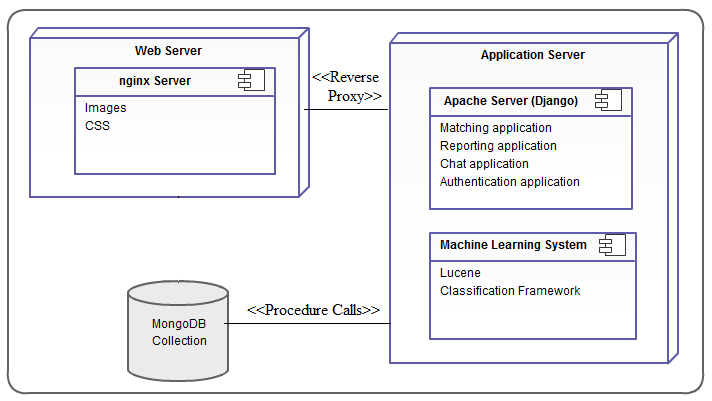
\includegraphics[width=150mm]{figs/deployment.png}
    \end{center}
        \caption[Deployment Diagram]{
        Deployment Diagram for \nplh.  Note that physical separation of the {\em nginx} server and the {\em Apache} server is optional.
	}
	 \label{fig:deployment}
\end{figure}

Because the application must serve a large amount of static files (mostly in the form of pictures, see Figure~\ref{fig:design3}), the primary web server which handles all direct requests is an {\em nginx}\footnote{http://www.nginx.org/} (``engine-X'') server.  This web server is generally more efficient at serving static files to clients, and is used in this setup to serve all static data (cascading style sheets, images, etc.); a reverse proxy is set up on a specific URL (typically the root Django application URL, i.e., ``/nplh/'') which forwards requests to an {\em Apache} server which hosts the Django installation via {\em mod\_wsgi}.

The Django installation used is actually a fork of version 1.4 which supports the use of non-relational databases in the data layer of Django.  The database driver used to support connectivity with MongoDB is an open-source driver known as {\em Django MongoDB Engine}, which provides object-relational mapping (ORM) for MongoDB collections as well as useful functionality like a map-reduce engine for common non-relational operations.

Within the Django deployment are several core system applications: the {\tt authentication}, {\tt chat}, {\tt reporting}, and {\tt matching} subsystems.  Although these applications make use of a common data store (described earlier in this chapter), they are loosely coupled and only refer to each other through URL redirection if necessary.  Modularization of the architecture is an important design goal to reduce development and maintenance complexity.

The following sections describe the implementation of each of these components; each section describes the purpose and functionality of the component and, in addition, provides a description of its implementation by specifying the the Django views (in MVC terminology, the controllers) included in the component.  In effect, these views describe the public interface of the applications.

\subsubsection {{\tt authentication} subsystem}

The {\tt authentication} subsystem includes functionality to handle all user-related tasks, such as user creation, authentication, linking accounts to existing social networks, importing social network data, and retrieving or editing user information.  The majority of the views contained in this application deal with the process of user authentication and tie in to Django's authentication mechanisms.  This subsystem, to a large extent, incorporates an open source Django application called {\em Django-Social-Auth}\footnote{https://github.com/omab/django-social-auth/}, which extends the default Django authentication system by supporting authentication via various third party providers.  \nplh{} utilizes the Twitter and Facebook authentication providers in order to both provide an efficient, easy-to-use account creation and authentication mechanism to users as well as harvesting relevant social connections from those accounts.  

The other features included this application further extend this functionality by providing a custom user model and additional functions and views.  The custom user model is necessary to reflect the {\tt User} artifact in Django's ORM by providing access to information like social reputation and a user's associated work items.  Other additions perform actions like retrieving a user's social connections and editing a user profile.  Table~\ref{table:authentication} details the views implemented in the {\tt authentication} subsystem.

\begin{table}[htb]
    \caption[Views provided by {\tt authentication} subsystem]{
	This table details the views provided by the {\tt authentication} application in terms of their arguments, HTTP method, purpose, and returned content.
	}
    \small
    \begin{center}
    % four columns - .25, .1, .15, .6
    \begin{tabularx}{ \textwidth}{| p{3cm} | p{1.2cm} | p{4cm} | X | } 
    \hline
    	Name (URL) & Method & Parameters & Purpose \\  \hline \hline

	{\tt auth}\textasteriskcentered \newline ({\tt /login/\newline(?P<backend>)/} )& GET, POST & backend [Object containing third party authentication information.] & Primary authentication method; accepts a string {\tt backend} that is used by a decorator to retrieve a third party service provider object.  This method uses this object to redirect the user to the appropriate third party authentication page.\\ \hline
	{\tt complete}\textasteriskcentered \newline ({\tt /complete/\newline(?P<backend>)/}) & GET & backend [Object containing third party authentication information.] & This method is fired upon a successful return from a third party authentication page; it creates the internal Django user and various session cookies, authenticating the user. \\ \hline
	{\tt associate} \textasteriskcentered \newline ({\tt /associate/\newline(?P<backend>)/}) & GET, POST &  backend [Object containing third party authentication information.] & Same as the {\tt auth} view, but attempts to associate a third party account with the currently authenticated user. \\ \hline
	{\tt associate_complete} \textasteriskcentered \newline ({\tt /associate/\newline complete/\newline(?P<backend>)/}) & GET &  backend [Object containing third party authentication information.] & This method is fired upon a successful return from a third party authentication page; it will associate the designated third party account with the current Django user. \\ \hline
	{\tt disconnect} \textasteriskcentered \newline ({\tt /disconnect/\newline(?P<backend>)/}) & GET &  backend [Object containing third party authentication information.] & Disconnects (deauthenticates) the user from the given third party provider; this may result in logging the user out. \\ \hline
	{\tt error} \newline ({\tt /error/}) & GET & None & This method is fired when an error is encountered in the authentication process.  Returns the user to a log in screen. \\ \hline
	{\tt profile} \newline ({\tt /profile/\newline(?P<username>)}) & GET & username [string] & Retrieves the specified user's (the current user if none is specified) profile page. \\ \hline
	{\tt profile} \newline ({\tt /profile/}) & POST & Form Data [object describing a user profile] & Updates the current user's profile information with relevant form data from POST values. \\ \hline
	
	\end{tabularx}
   \\ \rule{0mm}{5mm}
   \textasteriskcentered denotes functionality provided by the {\em django-social-auth} package. \newline
   URL format is the Django standard URL format (similar to regular expressions).
	\end{center}
	 \label{table:authentication}
\end{table}

\subsubsection {{\tt chat} subsystem}

The {\tt chat} subsystem includes functionality which facilitates communication between digital volunteers via chat rooms.  The backbone of this application is a third party Django application, {\em django-jqchat}\footnote{http://code.google.com/p/django-jqchat/}, which creates and manages chat rooms through standard HTTP interactions.  The client is shown a chat control (see the lower portion of Figure~\ref{fig:design1}) that is controlled and updated by simple asynchronous requests.  Although {\em django-jqchat} performs the majority of the work in this application, additional functionality has been added to better manage the creation of chat rooms, their association with other artifacts in the system, and the history of content generated in a chat room.  The two primary views (see Table~\ref{table:chat}) provided by this application's public interface are generally meant to be only called by asynchronous requests after initial page loads.  Making regular requests at a specified interval keeps this process fairly lightweight.  Using a solution which makes use of only Javascript is advantageous in that the server-side application code is integrated cleanly with the rest of the application, and in addition, the client is not burdened by a heavier implementation such as a Flash plugin. 

Chat rooms are automatically created when a pet report is first selected by a user in the matching interface.  This chat room is associated with the pet report and contains all the history of collaborative work on that report.  Although this functionality lives in this application, it is actually utilized by the {\tt matching} application.

The method by which contextual links (i.e., hypertext references that allow users to link to other artifacts in the system) are inserted into chat messages is implemented as an entirely client-side mechanism.  Javascript allows the user to drag and drop various visual controls (such as pet reports) to various locations on the matching interface; controls also have a link that appears on mouseover which, when clicked, will insert a contextual link into the user's chat message.  The link itself is then created via a standardized syntax that is transformed by additional Javascript into a hypertext link.  For example, after inserting a contextual link, the underlying string representation of a message might be, ``{\tt Check out this dog: \$\$pet:714\$\$}''.  The client-side Javascript would transform the latter part of this message based on the syntax {\tt pet:id} into the relative URL {\tt /nplh/matching/pet/714/} with display text of ``Pet-714''.  Table~\ref{table:translation} details the complete set of these transformations.

\begin{table}[htb]
		\caption[Translations performed client-side by {\tt chat} subsystem] {
		This table lists the various textual transformations done via Javascript to support contextual links to system artifacts in the chat control.
		}
		\begin{center}
		\begin{tabularx}{\textwidth}{| l | p{3cm} | X | l |}
		\hline
		Artifact & Syntax (Example) & Output URL & Output Text \\ \hline \hline
		Pet & {\tt pet:ID} \newline (\$\$pet:714\$\$) & {\tt /nplh/matching/pet/(ID)} & Pet-(ID) \\ \hline
		Match & {\tt match:ID} \newline (\$\$match:26\$\$) & {\tt /nplh/matching/match/(ID)} & Match-(ID) \\ \hline
		User & {\tt user:Username} \newline (\$\$user:josh\$\$) & {\tt /nplh/auth/profile/(Username)} & Username \\ \hline
		\end{tabularx}
		\\ \rule{0mm}{5mm}
		\end{center}
		\label{table:translation}
\end{table}

\begin{table}[htb]
    \caption[Views provided by {\tt chat} subsystem]{
	This table details the views provided by the {\tt chat} application in terms of their arguments, HTTP method, purpose, and returned content.
	}
    \begin{center}
    % four columns - .25, .1, .15, .6
    \begin{tabularx}{ \textwidth}{| p{3cm} | p{1.2cm} | p{4cm} | X | } 
    \hline
    	Name (URL) & Method & Parameters & Purpose \\  \hline \hline

	{\tt chat} \newline ({\tt /chat/(?P<id>)/\newline(?P<state>)/}) & GET & id [int] \newline state [int] & Retrieves the contents of the given chat room - if requested via an asynchronous call, the most recent contents (determined by comparing the provided state variable to the room's current state value) are returned via JSON message.  If the user is not a member of this chat room, the user is added to the members of this chat room.\\ \hline
	{\tt chat} \newline ({\tt /chat/\newline(?P<id>)/}) & POST & id [int] \newline Form Data [object containing chat message] & Called when a user posts a message to a chat room.  The content of the chat room is updated and the room's state is incremented. \\ \hline

	\end{tabularx}
   \\ \rule{0mm}{5mm}
   
	\end{center}
	 \label{table:chat}
\end{table}

\subsubsection {{\tt reporting} subsystem}

The {\tt reporting} subsystem includes functionality to allow users to submit and edit lost or found pet reports.  While this functionality caters to the data scout user, the editing component is open is more focused on the remote volunteer.  The core views in this application are listed in Table~\ref{table:reporting}.

This application, in addition to housing the primary data generation mechanisms for the system, also incorporates interaction with the machine learning system in the form of providing training examples for the {\tt Pet} classifier (discussed in the next chapter).  This interaction occurs when a new pet report is submitted (it becomes indexed in the information retrieval system) and when it is edited or upvoted.  Upvoting a pet indicates a value judgment on the quality and completeness of that pet report (users are directed to make this kind of assessment based on provided instructions), and marks the pet report as a positive training example for the classifier.  Editing a pet report indicates some kind of deficiency in the original report; the edited report is submitted as a positive training example.  The original report can be compared with the newly edited report - the differences between them can be used as a negative training example.

\begin{table}[htb]
    \caption[Views provided by {\tt reporting} subsystem]{
	This table details the views provided by the {\tt reporting} application in terms of their arguments, HTTP method, purpose, and returned content.
	}
    \begin{center}
    % four columns - .25, .1, .15, .6
    \begin{tabularx}{ \textwidth}{| p{3cm} | p{1.2cm} | p{4cm} | X | } 
    \hline
    	Name (URL) & Method & Parameters & Purpose \\  \hline \hline

	{\tt report} \newline ({\tt /report/}) & GET & state [int] & Displays a form allowing the user to submit a lost or found pet report, attaching relevant information (breed, color, description, etc.) and pictures.\\ \hline
	{\tt report} \newline ({\tt /report/}) & POST & Form Data [object describing pet report] & Validates and processes a submitted pet report, creating a {\tt Pet} artifact if successful.  Returns a confirmation page.\\ \hline
	{\tt edit} \newline ({\tt /report/edit/\newline(?P<id>)/}) & GET & id [int] & Retrieves the specified pet report and displays a form to the user which allows the user to edit the report or vote on the quality of the report.\\ \hline
	{\tt edit} \newline ({\tt /report/edit/\newline(?P<id>)/}) & POST & id [int] \newline Form Data [object describing pet report] & Makes changes to the specified pet report using form data.  Submits the changed report for training to the machine learning system.\\ \hline
	{\tt upvote} \newline ({\tt /report/upvote/\newline(?P<id>)/}) & POST & id [int] & Records an upvote from the current user for the specified pet report.  Submits the report for training to the machine learning system.\\ \hline

	\end{tabularx}
   \\ \rule{0mm}{5mm}
   
	\end{center}
	 \label{table:reporting}
\end{table}

\subsubsection {{\tt matching} subsystem}

The {\tt matching} subsystem is the heart of \nplh.  It facilitates the entire matching task work flow, which includes the two primary user interfaces in the system.  In addition, the application also facilitates the verification work flow, which involves checkers voting on proposed matches.  When a match receives enough votes, the contacts on each pet report in the match are notified to perform final verification; after this final verification, the pet reports are removed from circulation.  These two activities represent the bulk of the work done in the system (the only other major activity, the reporting of lost or found pets, being catered to by the {\tt reporting} subsystem).  Table~\ref{table:matching} details the views contained in this subsystem.

It also features significant interactions with every other component of the system; in particular, it is the application which is the primary collaborator with the machine learning components of the system.  When users select a pet to work on and enter the primary matching interface (see Figure~\ref{fig:design4} for a prototype of this interface), the {\tt matching} application uses that pet as a query to the machine learning system.  The machine learning system produces a ranked list of suggested matches which is used directly to output a selection of pets to the user.  Furthermore, whenever a match is confirmed (and taken out of circulation), it is presented as training data to the {\tt Match} classifier.

\begin{table}[htb]
    \caption[Views provided by {\tt matching} subsystem]{
	This table details the views provided by the {\tt matching} application in terms of their arguments, HTTP method, purpose, and returned content.
	}
    \begin{center}
    % four columns - .25, .1, .15, .6
    \begin{tabularx}{ \textwidth}{| p{5cm} | l | p{2.5cm} | X | } 
    \hline
    	Name (URL) & Method & Parameters & Purpose \\  \hline \hline

	{\tt pet} \newline ({\tt /matching/pet/\newline(?P<id>)/}) & GET & id [int] & Displays a detailed view of the specified pet report.  This view is generally used in AJAX calls to display a pop up form with the pet's information.\\ \hline
	{\tt match} \newline ({\tt /matching/match/\newline(?P<id>)/}) & GET & id [int] & Displays a detailed view of the specified match.  This view is generally used in AJAX calls to display a pop up form with the match's information.\\ \hline
	{\tt vote_match} \newline ({\tt /matching/match/\newline(?P<id>)/}) & POST & id [int] \newline Form Data [boolean for up or down vote] & Records the vote (positive or negative) of the current user for the specified match.\\ \hline
	{\tt home} \newline ({\tt /}) & GET & None & This view acts as the home page for the application; it displays the first screen of the matching interface, where a user selects a pet to work on.\\ \hline
	{\tt matches} \newline ({\tt /matching/matches/}) & GET & None & This view acts as the match verification page; returns a page containing all the current proposed matches.\\ \hline
	{\tt matching} \newline ({\tt /matching/(?P<id>)/}) & GET & id [int] & After selecting a pet to work on (from the detailed view), this view retrieves the information necessary to create the matching interface for that pet.  This view interacts with the machine learning system to retrieve the suggested list of matches.\\ \hline
	{\tt propose_match} \newline ({\tt /matching/match/\newline(?P<id_lost>)/\newline(?P<id_found)})/ & POST & id_lost [int] \newline id_found [int] & Proposes a match between the two specified pet reports and creates a {\tt Match} artifact.\\ \hline	
		\end{tabularx}
   \\ \rule{0mm}{5mm}
	\end{center}
	 \label{table:matching}
\end{table}

\subsubsection {{\tt Machine Learning} subsystem}

The {\tt Machine Learning} subsystem is not actually a Django application (i.e., it has no views) but instead acts as the public interface for accessing the machine learning components of the system.  This system is more thoroughly examined in Chapter 4, but the public interface for the software is presented here.  This interface presents functionality that allows the rest of the system to be agnostic to the underlying details of the machine learning components, which are the parts of this system that are most likely to change and evolve over time.

The public interface is focused on two types of activity: requesting a ranked list of pet matches for a given query (pet report) and providing an artifact to the machine learning system for retraining.  The latter activity is interesting as it can be viewed as presenting observations of user activity to the machine learning components.  Table~\ref{table:ml} presents the public interface of this application in a similar fashion to the previous sections, but again, note that this application is not a Django application.

\begin{table}[htb]
    \caption[Public interface for {\tt Machine Learning} subsystem]{
	This table details the public interface of the {\tt Machine Learning} subsystem.  These are pure Python methods, and do not represent a Django application.  The design and implementation of this system is described in the following chapter.
	}
    \begin{center}
    \begin{tabularx}{ \textwidth}{| l | p{4cm} | X | } 
    \hline
    	Method Name & Parameters & Purpose \\  \hline \hline
		{\tt train_pet} & pet [{\tt Pet}] \newline positive [boolean] & Provides a {\tt Pet} artifact as a training example to the {\tt Pet} classifier.  The boolean parameter indicates whether this is a positive or negative example. \\ \hline
		{\tt train_match} & match [{\tt Match}] \newline positive [boolean] & Provides a {\tt Match} artifact as a training example to the {\tt Match} classifier.  The boolean parameter indicates whether this is a positive or negative example. \\ \hline
		{\tt query} & pet [{\tt Pet}] & Queries the information retrieval and classifier systems for a list of pets that most closely correspond to the provided pet.  These form a ranked list that is used in the {\tt matching} subsystem. \\ \hline		
	 \end{tabularx}
   \\ \rule{0mm}{5mm}

	\end{center}
	 \label{table:ml}
\end{table}